\chapter{Annuities with non-contigent payments}
\label{chapter_annuity}


\begin{definition}
\label{definition:annuity}
An annuity is a series of payments made at equal time intervals. 
\end{definition}

    Types of Annuities (Based on Payment Structure)
\begin{comments}
\begin{enumerate}
  \item \textbf{Amount of Payments}
  \begin{itemize}
    \item \textbf{Level payments}: Equal payment each period
    \item \textbf{Non-level payments}: Varying payment amounts
  \end{itemize}
  
  \item \textbf{Timing of Payments}
  \begin{itemize}
    \item \textbf{Immediate annuity}: Payment at \textit{end} of each period
    \item \textbf{Due annuity}: Payment at \textit{beginning} of each period
  \end{itemize}
  
  \item \textbf{Number of Payments}
  \begin{itemize}
    \item \textbf{Term annuity}: Fixed number of payments
    \item \textbf{Perpetuity}: Payments continue \textit{forever}
  \end{itemize}
  
  \item \textbf{Deferral of Payments}
  \begin{itemize}
    \item \textbf{Deferred annuity}: Payments start \textit{after a delay}
  \end{itemize}
\end{enumerate}
\end{comments}


\section{Level annuity} 
\subsection{Immediate Annuity}

Consider a level annuity-immediate where each payment is \textbf{1 unit}, made at the \textbf{end of each period}. There are 
n total payments, and the effective rate of interest  \textbf{per unit of time} is \textbf{\( i \)}. One unit of time equals one period.

\begin{center}
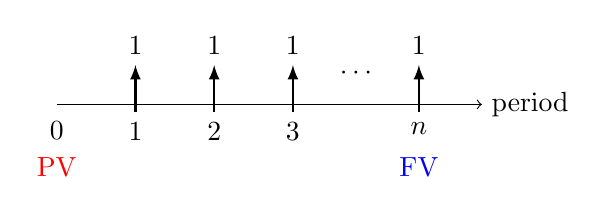
\begin{tikzpicture}
\draw[->] (0,0) -- (5.4,0)node[right]{period};

\foreach \X in {0,1,2,3} {
  \ifnum\X=0
    % Just draw label at x=0, no arrow
    \draw (\X,-0.1) node[below]{$\X$};
  \else
    % For x > 0, draw arrow and value 1
    \draw[thick,-latex] (\X,-0.1) node[below]{$\X$} -- ++(0,0.6) node[above]{$1$};
  \fi}
\draw[thick,-latex] (4.6,-0.1) node[below]{$n$} -- ++(0,0.6) node[above]{$1$};
\node at (3.8,0.4) {$\cdots$};
  \node[red] at (0,-0.8) {PV};
\node[blue] at (4.6,-0.8) {FV};
\end{tikzpicture}
\end{center}
\begin{comments}
The present value (sum of discounted payments) of that annuity at period t=0 is defined as:

\[
PV = \frac{1}{1+i} + \frac{1}{(1+i)^2} + \cdots + \frac{1}{(1+i)^n} = \sum_{k=1}^{n} \frac{1}{(1+i)^k} = \frac{1 - v^n}{i}, \quad \text{where } v = \frac{1}{1+i}
\]

The future value (value at time n) of the same annuity is:
\[FV = 1 + (1 + i) + (1 + i)^2 + \cdots + (1 + i)^{n-1} = \sum_{k=0}^{n-1} (1 + i)^k\]

\end{comments}



\begin{formula}\label{immediate_annuity}(Immediate Annuity)

\[a_{\angl{n} i} = PV = \frac{1 - v^n}{i}, \quad \text{where } v = \frac{1}{1+i}
\]

\[s_{\angl{n} i} = FV = \sum_{k=1}^{n} (1 + i)^k =  \frac{(1+i)^n - 1}{i}\]


\end{formula}

\subsection{Annuity Due}

Consider a level annuity-due where each payment is \textbf{1 unit}, made at the \textbf{beginning of each period}. There are 
n total payments, and the effective rate of interest \textbf{per unit of time} is \textbf{\( i \)}. One unit of time equals one period.

\begin{center}
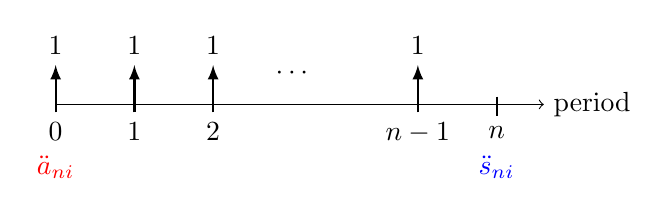
\begin{tikzpicture}
 \draw[->] (0,0) -- (6.2,0) node[right]{period};

 \foreach \X in {0,1,2} {
 \draw[thick,-latex] (\X,-0.1) node[below]{$\X$} -- ++(0,0.6) node[above]{$1$};}
 \draw[thick,-latex] (4.6,-0.1) node[below]{$n-1$} -- ++(0,0.6) node[above]{$1$};
\draw[thick] (5.6,0.1) -- (5.6,-0.15) node[below]{$n$};
 \node at (3.0,0.4) {$\cdots$};
 
 \node[red] at (0,-0.8) {$\ddot{a}_{\angl{n} i}$};
 \node[blue] at (5.6,-0.8) {$\ddot{s}_{\angl{n} i}$};
\end{tikzpicture}
\end{center}
\begin{comments}
\par The present value (sum of discounted payments) of that annuity at period t=0 is:

\[
PV = 1 + \frac{1}{1+i} + \frac{1}{(1+i)^2} + \cdots + \frac{1}{(1+i)^{n-1}} = \sum_{k=0}^{n-1} \frac{1}{(1+i)^k} = \frac{1 - v^n}{i} \cdot (1 + i), \quad \text{where } v = \frac{1}{1+i}
\]

The future value (value at time n) of the same annuity is:
\[FV = (1 + i) + (1 + i)^2 + \cdots + (1 + i)^n = \sum_{k=1}^{n} (1 + i)^k
\]

\end{comments}

\begin{formula}\label{annuity_due}(Annuity Due)

\[\ddot{a}_{\angl{n} i} = PV = \frac{1 - v^n}{i} \cdot (1 + i) = \frac{1 - v^n}{d}, \quad \text{where } d = \frac{1+i}{i}
\]

\[\ddot{s}_{\angl{n} i} = FV = \sum_{k=1}^{n} (1 + i)^k\]

\end{formula}


\section{Varrying-Payments Annuity}
\begin{definition}
    Payments in an annuity that changes instead of staying level.
\end{definition}

\subsection{Payments in Arithmetic Progression}
\subsubsection{1. Arithmetic Increasing Annuity}

\begin{comments}
Let the first payment = \textbf{P}, each following payment increases by \textbf{Q}, and there are total \textbf{n} payments. 

\begin{center}
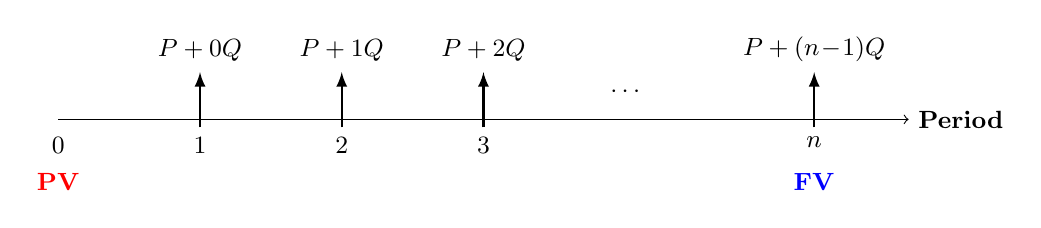
\begin{tikzpicture}[xscale=1.2, font=\small] % Wider and smaller font
  \draw[->] (0,0) -- (9,0) node[right]{\textbf{Period}}; % Extended width
  
  % Period labels (0 to n)
  \foreach \X in {0,1,2,3} {
    \draw (\X*1.5,-0.1) node[below]{$\X$}; % Spaced every 2 units
  }
  \draw (8,-0.1) node[below]{$n$}; % 'n' at far right
  
  % Payments (P, P+Q, P+2Q, ..., P+(n-1)Q)
  \foreach \X [count=\Y from 0] in {1,2,3} {
    \draw[thick, -latex] (\X*1.5,-0.1) -- ++(0,0.7) 
      node[above, align=center]{$P + \Y Q$}; % \Y starts at 0
  }
  \draw[thick, -latex] (8,-0.1) -- ++(0,0.7) 
    node[above, align=center]{$P + (n\!-\!1)Q$}; % Last payment
  
  % Dots for continuation
  \node at (6,0.35) {$\cdots$};
  
  % PV/FV labels
  \node[red] at (0,-0.8) {\textbf{PV}};
  \node[blue] at (8,-0.8) {\textbf{FV}};
\end{tikzpicture}
\end{center}

\end{comments}

\begin{formula}
(Arithmetic Increasing Annuity) \\
Present Value at time (period) t=0: 
\[
PV = P \cdot a_{\overline{n}|i} + Q \cdot \frac{a_{\overline{n}|i} - n \cdot v^n}{i}
\] 
Accumulated Value at time (period) t=n: 
\[
AV = P \cdot s_{\overline{n}|i} + Q \cdot \frac{s_{\overline{n}|i} - n}{i}
\]
\end{formula}\leavevmode\newline




\subsubsection{2. Increasing Annuity}
\begin{comments}
When P=Q=1, payments become 1,2,...,n. 

    \begin{center}
\begin{tikzpicture}[xscale=1.2, font=\small]
  \draw[->] (0,0) -- (9,0) node[right]{\textbf{Period}}; % Timeline
  
  % Period labels (0 to n)
  \foreach \X in {0,1,2,3} {
    \draw (\X*1.5,-0.1) node[below]{$\X$}; % Spaced every 2 units
  }
  \draw (8,-0.1) node[below]{$n$}; % Last period
  
  % Increasing payments (1, 2, 3,..., n)
  \foreach \X in {1,2,3} {
    \draw[thick, -latex] (\X*1.5,-0.1) -- ++(0,0.7) 
      node[above]{$\X$}; % Payment amounts
  }
  \draw[thick, -latex] (8,-0.1) -- ++(0,0.7) 
    node[above]{$n$}; % Last payment
  
  % Dots for continuation
  \node at (6,0.35) {$\cdots$};
  
  % Labels
  \node[red] at (0,-0.8) {\textbf{PV}};
  \node[blue] at (8,-0.8) {\textbf{FV}};
  
\end{tikzpicture}
\end{center}

\end{comments}

\begin{formula} 
(Increasing Annuity) \\
PV at time (period) t = 0: \[\quad (Ia)_{\angl{n}i} = a_{\angl{n}i} + \frac{a_{\angl{n} i} - nv^n}{i}  = \frac{(1+i)a_{\angl{n}i - nv^n}}{i} = \frac{\ddot{a}_\angl{n} i - nv^n}{i} \] 

FV at time (period) t = n: 
\[ \quad (Is) _{\angl{n} i} = (1+i)^n \cdot (Ia)_{\angl{n} i} = \frac{\ddot{s}_{\angl{n}i} - n}{i} = \frac{s_{\angl{n+1} i } - (n + 1)}{i}
\]

\end{formula} 

\leavevmode\newline




\subsubsection{3. Decreasing Annuity}
\begin{comments}
When P=n and Q=1, payments become n, n-1, n-2, ..., 1.

    \begin{center}
\begin{tikzpicture}[xscale=1.2, font=\small]
  \draw[->] (0,0) -- (9,0) node[right]{\textbf{Period}}; % Timeline
  
  % Period labels (0 to n)
  \foreach \X in {0,1,2,3} {
    \draw (\X*1.5,-0.1) node[below]{$\X$}; % Spaced every 1.5 units
  }
  \draw (8,-0.1) node[below]{$n$}; % Last period
  
  % Decreasing payments (n, n-1, n-2,..., 1)
  \foreach \X [evaluate=\X as \Y using {int(4-\X)}] in {1,2,3} {
    \draw[thick, -latex] (\X*1.5,-0.1) -- ++(0,0.7) 
      node[above]{$n\!-\!\Y$}; % Payment amounts (n-1, n-2, etc.)
  }
  \draw[thick, -latex] (8,-0.1) -- ++(0,0.7) 
    node[above]{$1$}; % Final payment
  
  % Dots for continuation
  \node at (6,0.35) {$\cdots$};
  
  % Labels
  \node[red] at (0,-0.8) {\textbf{PV}};
  \node[blue] at (8,-0.8) {\textbf{FV}};

\end{tikzpicture}
\end{center}
\end{comments} 

\begin{formula}
(Decreasing Annuity) \\
\[
\text{PV}_{t=0} = (Da)_{\angl{n}} = n a_{\angl{n}i} - \frac{a_{\angl{n}i} - n v^n}{i} 
= \frac{n - n v^n - a_{\angl{n}i} + n v^n}{i} 
= \frac{n - a_{\angl{n}i}}{i}
\]

\[
\text{FV}_{t=n} =  (Ds)_{\angl{n}} = (1+i)^n (Da)_{\angl{n}} 
= \frac{n(1+i)^n - s_{\angl{n}i}}{i} 
= (n+1)a_{\angl{n}i} - (Ia)_{\angl{n}i}
\]
\end{formula}

%-------------------------------------------

\subsubsection{4. Varying Perpetuity-Immediate with Arithmetic growth}
\begin{comments}
    The payments follow an Arithmetic progression with constants P \> 0 and Q \> 0. Payments are P, P+Q, P+2Q,... First payment is at the end of first period. \\


Present Value of Perpetuity-Immediate with payments of arithmetic progression: \\
\[
\text{PV} = \lim_{n \to \infty} \left( P a_{\angl{n}} + Q \cdot \frac{a_{\angl{n}} - n \nu^n}{i} \right)
\]

Since n goes to infinity, 
\[
\lim_{n \to \infty} a_{\angl{n}} = a_{\angl{\infty}} = \frac{1}{i}
\]
\[
\lim_{n \to \infty} n \nu^n = 0 \quad \text{(via L'Hôpital's Rule)}
\]

Hence, 
\[
\text{PV} = \frac{P}{i} + \frac{Q}{i^2}
\]

\end{comments}
\begin{formula} (Increasing Perpetuity-Immediate - Arithmetic Growth) \\
When $P = Q = 1$:
\[
(Ia)_{\angl{\infty}} = \frac{1}{i} + \frac{1}{i^2}
\]
\end{formula}


\begin{table}[]
        \centering
        \begin{tabular}{|| c | c | c ||}
        \hline \hline
          Annuity &  PV & FV\\
        \hline \hline
        Arithmetic Increasing Annuity &
$P \cdot a_{\overline{n}|i} + Q \cdot \frac{a_{\overline{n}|i} - n \cdot v^n}{i}$ &
$P \cdot s_{\overline{n}|i} + Q \cdot \frac{s_{\overline{n}|i} - n}{i}$ \\
\hline \hline
    \end{tabular}
    \caption{Summary}
    \label{tab:my_label}
\end{table}

%-----------------------------------------------------
\subsubsection{5. Varying Perpetuity-Due with Arithmetic growth}
\begin{comments}
  The PV of a perpetuity-immediate with arithmetic growth is: 
  \[
    \text{PV}_{\text{immediate}} = \frac{P}{i} + \frac{Q}{i^2}
  \]

  For perpetuity-due, we shift everything 1 period earlier: 
  \[
      \text{PV}_{\text{due}} = (\frac{P}{i} + \frac{Q}{i^2})(1+i) = (\frac{1}{i} + \frac{1}{i^2})(1+i) = \frac{(1+i)^2}{i^2} = \frac{1}{d^2}
  \]

\end{comments}


\begin{definition}
    (Increasing Perpetuity-Due - Arithmetic Growth)
When P = Q = 1:
\[
  (I\ddot{a})_{\angl{\infty}} = \frac{1}{d^2}
\]
  \end{definition}



%-----------------------------------------------------
\subsection{Payments in Geometric Progression}
\begin{definition}
    A \textbf{geometric annuity} has \textbf{n payments}, each payment grows by a constant percentage, or \textbf{growht rate k}. 
    If the first payment is 1, and growth rate is $k$, then the payments are 
    \[
      \text{Payments} = 1, (1+k), (1+k)^2, \dots , (1+k)^{n-1}
    \]  
\end{definition}
\begin{comments}
For each payment in n payments of the annuity, each is discounted back to time 0 by discount factor $\frac{1}{1+i}$. 
\begin{align*}
    PV &= v + v^2 (1 + r) + \dots + v^n (1 + k)^{n-1} \\
    &= v (1 + v(1+k) + \dots + v^{n-1}(1+k)^{n-1}) \\
\end{align*}
\begin{comments}
  The RHS follows a geometric series with common ratio $r = \frac{1+k}{1+i}$, hence its sum follows: 
\end{comments}
\begin{align*}
    \text{PV} &= v \left[ \frac{1 - \left( \frac{1 + k}{1 + i} \right)^n}{1 - \frac{1 + k}{1 + i}} \right]  = v \left[ \frac{1 - \left( \frac{1 + k}{1 + i} \right)^n}{\frac{i - k}{1 + i}} \right] \\
    &= v \left[ \frac{1 - \left( \frac{1 + k}{1 + i} \right)^n}{v(i - k)} \right] =\frac{1 - \left( \frac{1 + k}{1 + i} \right)^n}{i - k}
\end{align*}

\begin{formula} (PV of an annuity-immediate of geometric progression)
  \[
  \text{PV} = \frac{1 - \left( \frac{1 + k}{1 + i} \right)^n}{i - k}
  \]
\end{formula}


%---------------------------------
\begin{example}(Geometric annuity with unknown interest rate)
    A 10-year annuity-immediate has:
\begin{itemize}
    \item First payment: \$11
    \item Subsequent payments: 10\% increase each year
    \item Accumulated value: \$220.8
\end{itemize}
Find the annual effective interest rate $i$.
\begin{enumerate}
    \item \textbf{AV as Geometric Series:}
    \[
    AV = 11(1.1)^9 \left[1 + \frac{1+i}{1.1} + \left(\frac{1+i}{1.1}\right)^2 + \cdots + \left(\frac{1+i}{1.1}\right)^9 \right]
    \]
    
    \item \textbf{Sum the Series:}
    \[
    220.8 = 11(1.1)^9 \cdot \frac{1 - \left(\frac{1+i}{1.1}\right)^{10}}{1 - \frac{1+i}{1.1}}
    \]
    
    \item \textbf{Substitute Values:}
    \[
    220.8 = 25.937 \cdot \frac{1 - (1 + j)^{10}}{-j}, \quad j = \frac{1.1}{1+i} - 1
    \]
    
    \item \textbf{Solve for $j$:}
    \[
    \frac{(1 + j)^{10} - 1}{j} = 8.513 \implies j \approx 0.03773
    \]
    
    \item \textbf{Find $i$:}
    \[
    j = \frac{1.1}{1+i} - 1 \implies i = \boxed{0.06} \ (6\%)
    \]
\end{enumerate}
\end{example}
\end{comments}




%-------------------------------------------------------------------
\section{Deferred Annuity}
\begin{definition}
    A deferred annuity is an annuity where the payments start at a future date, not immediately.
\end{definition}

\begin{comments}
    There are 2 parts in a deferred annuity: 
    \begin{enumerate}
        \item Deferral period: Time you wait before payments start.
        \item Payment period: Regular payments begin (like a normal annuity).
    \end{enumerate} 
    \break

    Three annuity valuation cases: 
    \begin{itemize}
        \item \textbf{Before 1st Payment (Deferred Annuity)}: $PV=v^m a_{\angl{n}i} = a_{\angl{m+n}i} - a_{\angl{m}i}$
        \item \textbf{After Last Payment}: AV = move future value forward using interest.
        \item \textbf{Between Payments}: Split into past and future parts: some payments made, some still due.
    \end{itemize}
\end{comments}
\begin{comments}
Calculate the present value of the \( n \)-period annuity (\( a_n \)) as if payments were starting now. Then discount it back \( m \) periods using \( v^m = (1 + i)^{-m} \).
\end{comments} \\

%------------------------------------
\subsection{PV before first payment of an annuity-immediate}

\begin{theorem}
The present value is:
$\text{PV} = v^m a_n$
\end{theorem}


\begin{figure}
  \centering
  \includegraphics[width=1.0\linewidth]{images/deferred_annuity.JPG}
  \caption{Deferred Annuity}
  \label{fig:enter-label}
\end{figure}


\begin{comments}
    We proof the above theorem by derviving from standard annuity formulas: \\

    $a_{\angl{m+n}i}$ is the PV of an annuity-immediate including all payments over m+n periods (at this point, we assume that there are m+n payments from period t=1 to t=m+n but the actual number of payments is only n, as in 0-m period, there are zero payments).\\
    
    $a_{\angl{m}i}$ is the PV of an annuity-immediate over m periods with m payments (this is an assumption as in reality there is zero payment at this point since this is the deferred period). 
\end{comments}

\begin{proof}
    \[
a_{\angl{m+n}i} - a_{\angl{m}i} = \frac{1 - \nu^{m+n}}{i} - \frac{1 - \nu^m}{i}
\]

\[
= \frac{\nu^m - \nu^{m+n}}{i}
= \frac{\nu^m (1 - \nu^n)}{i}
= \nu^m a_n
\]

\[
\Rightarrow a_{\angl{m+n}i} - a_{\angl{m}i} = v^m a_n
\]

This means:
\begin{itemize}
    \item Calculate the present value of the \( n \)-period annuity (\( a_n \)) at time t=m (1st payment starts at time t=m+1. 
    \item Then discount it back \( m \) periods using \( v^m = (1 + i)^{-m} \).
\end{itemize}

Note: those expressions are for convinient calculation.

\end{proof}
%--------------------------------
\section{Varying-Interest Annuity}
\begin{definition}
    An annuity has an interest that can vary in each period. Let $i_k$ be the interest rate from time k-1 to k. 
\end{definition}

\subsection{Rate $i_k$ is applied for period k (date depends on calender year)}
\begin{comments}
    Starting from when the 1st payment made at time 0, up to time $k^{th}$ or later, the future payments are discounted/accumulated using \textbf{all previous rate} $i_1, i_2, i_3,...,i_k$. \\
\end{comments}


\subsubsection{Annuity-immediate}
\begin{comments}

    The PV of an annuity-immediate is: 
    \[ a_{\angl{n}i} = \frac{1}{1 + i_1} + \frac{1}{(1 + i_1)(1 + i_2)} + \cdots + \frac{1}{(1 + i_1)(1 + i_2) \cdots (1 + i_n)} \] \\
    The AV of an anntuiy-immediate is:
    \[ s_{\angl{n+1}i} = \ddot{s}_{\angl{n}i} + 1 \] \\
\end{comments}


\subsubsection{Annuity-due}
\begin{comments}
    The PV of an annuity-due is:
    \[ \ddot{a}_{\angl{n}i} = 1 + a_{\angl{n-1}i} \] 
    The AV of an anntuiy-due is: 
    \[ \ddot{s}_{\angl{n}i} = (1 + i_1)(1 + i_2)\cdots(1 + i_n) + \cdots + (1 + i_{n-1})(1 + i_n) + (1 + i_n) \]
\end{comments}


\subsection{Rate $i_k$ is applied for period k and before/later (rate depends on deposit time)}

\begin{comments}
    Regardless of when the payments are made, any payments in the period $k$ is discounted using only rate $i_k$. 
    The rate $i_k$ is the effective rate for period $i\leq k$ (PV) and $i\ge k$.  Intuition: The rate depends on 
    when you invest - it locks in the rate. 
\end{comments}


\subsubsection{Annuity-Immediate}
The PV of an annuity-immediate is:  

\[ a_{\angl{n}i} = \frac{1}{(1 + i_1)^1} + \frac{1}{(1 + i_2)^2} + \cdots + \frac{1}{(1 + i_n)^n}\]
The FV of an annuity-immediate is:  
\[s_{\angl{n+1}i} = \ddot{s}_{\angl{n}i} + 1 \]

\subsubsection{Annuity-due}
The PV of an annuity-due is:
\[\ddot{a}_{\angl{n}i} = 1 + a_{\angl{n-1}i}\]
The FV of an annuity-due is:
\[\ddot{s}_{\angl{n}i} = (1 + i_1)^n + (1 + i_2)^{n-1} + \cdots + (1 + i_n)^1\]




%------------------------------------------------------------
\section{Non-coinciding Frequencies Annuity}
\begin{definition}
    An annuity where \textbf{payments} made and \textbf{interest} compounded at a different frequency. 
    \[
      (1+j)^m = (1+i)^n
    \]

    \begin{itemize}
      \item $j$ = rate per payment period (what we want)
      \item $m$ = number of payment periods
      \item $i$ = rate per compounding period 
      \item $n$ = number of compounding periods 
    \end{itemize}
\end{definition}

\begin{comments}
  \begin{center}
  \begin{tabular}{>{\centering\arraybackslash}m{1.5cm} >{\centering\arraybackslash}m{2.5cm} >{\centering\arraybackslash}m{4cm} >{\centering\arraybackslash}m{4cm}}
  \toprule
  \textbf{Term} & \textbf{Applies To} & \textbf{Rate For} & \textbf{Found From} \\ 
  \midrule
  $i$ & Compounding frequency & Compounding periods (e.g., quarterly) & Given by nominal rate \\ 
  \addlinespace
  $j$ & Payments frequency & Payment periods (e.g., monthly) & Must be \textbf{calculated} to match payment frequency \\ 
  \bottomrule
  \end{tabular}
  \end{center}
\end{comments}

\begin{formula}
  If \textbf{nominal rate $i_{\text{nom}}$} is compounded $n$ times per year, then: 
  \[
    i_{\text{eff}} + 1 = (1+\frac{i_{\text{nom}}}{n}) 
  \]
\end{formula}









%-------------------------------------
\section{Perpetuity}

\begin{definition}
  Perpetuity is an annuity that pays forever. Perpetuity-immediate has payments start 1 period from now.
  Perpetuity-due has payments which start immediately (now).
\end{definition}

\begin{formula} (Present Value)

  Perpetuity-Immediate: 
    \[
      \text{PV} = \text{a}_{\angl{\infty}} = v + v^2 + \dots = \frac{1}{i}
    \]
  
  Perpetuity-Due: 
  \[
    \text{PV} = \ddot{a}_{\angl{\infty}} = 1 + v + v^2 + \dots = \frac{1}{d}
  \]

  Relationship: $\ddot{a}_{\angl{\infty}} = 1 + \text{a}_{\angl{\infty}}$
\end{formula}

